\documentclass[nochap,palatino,notitlepage]{apuntes}

\title{Organización de Empresas Tecnológicas}
\author{Guillermo Julián}
\date{15/16 C1}

% Paquetes adicionales
\usepackage{fancysprefs}
\usepackage{booktabs}
\usepackage{multirow}
\usepackage{textcomp}

\begin{document}
\pagestyle{plain}
\maketitle

\begin{abstract}
Estos apuntes pretenden ser un resumen concreto y más o menos completo de la asignatura de Organización de Empresas Tecnológicas, con (esperemos) pocas abreviaturas.
\end{abstract}

\tableofcontents
\newpage
\section{Empresa}

\subsection{Introducción}

A grandes rasgos, una \concept{Empresa} es una organización con ánimo de lucro, propiedad de una o varias personas físicas o jurídicas (una \concept{Persona\IS jurídica} es una empresa o entidad). El control de la empresa lo ejercen los propietarios, que se organizan en un consejo de administración. En el día a día, los directivos son los que dirigen la empresa.

Las empresas se pueden constituir en dos formas principalmente: como \concept{Sociedad\IS Anónima} o como \concept{Sociedad\IS Limitada}, ambas reguladas por el \href{https://www.boe.es/buscar/act.php?id=BOE-A-2010-10544}{RD 1/2010 de 2 de julio}. Ambas tienen también versiones unipersonales. La principal diferencia está en la propiedad y en cómo se distribuye el capital social. En la SL, los socios ponen un mínimo de 3.000 euros, desembolsado completamente en el momento de la constitución. Además, no pueden vender libremente sus participaciones (los estatutos ponen las normas), salvo a familiares directos.

Por el contrario, las sociedades anónimas tienen acciones (no participaciones) al portador, que se pueden vender y comprar libremente (por eso sólo las SA cotizan en bolsa). Lo malo es que el capital mínimo es mayor, de 60.000 euros, aunque sólo hay que desembolsar un 25 \% en el momento de la constitución.

Las empresas pagan impuestos a través del Impuesto de Sociedades y de la Seguridad Social. Si la empresa quiebra, sólo se responde con el patrimonio de la empresa y no con el de los socios (al contrario que si una persona es un autónomo\footnote{También conocidos como Pringados\texttrademark.}, que responde de las deudas con todo su patrimonio).

En cualquiera de los dos casos, es importante ver la relación laboral que tienen los directivos y administradores con la empresa. Los altos directivos\footnote{Los que ejercitan poderes que corresponden a los titulares de la empresa, y con autonomía y plena responsabilidad limitadas únicamente por los órganos de gobierno de la empresa.} tienen una relación de carácter especial con la empresa, no regulada por el \href{https://www.boe.es/buscar/act.php?id=BOE-A-1995-7730&tn=1&vd=&p=20151024}{Estatuto de los trabajadores} sino por el \href{https://www.boe.es/diario_boe/txt.php?id=BOE-A-1985-17006}{Real Decreto 1382/1985}, aunque a efectos prácticos el contrato es un contrato laboral. Sin embargo, si los altos directivos realizan tareas de administración o gerencia en la empresa (por ejemplo, consejeros), ya no hay relación laboral sino mercantil, y por lo tanto el directivo en cuestión debe darse de alta en el régimen de autónomos.

\subsubsection{Creación de una empresa}

Para crear una empresa, hay que seguir la burocracia correspondiente. En general, hay que seguir los siguientes pasos, sacados de la \href{http://www.creatuempresa.org/es-ES/PasoApaso/}{página del Ministerio de Industria}.

\begin{enumerate}
\item Ir al Registro Mercantil para acreditar que no hay otra sociedad con el mismo nombre que la que queremos constituir.
\item Ir a la AEAT\footnote{Agencia Estatal de Administración Tributaria, también llamada Agencia Tributaria o Hacienda.} a obtener un CIF provisional.
\item Ir al banco y desembolsar el capital social en una cuenta a nombre de la empresa (para esto necesitamos el CIF provisional).
\item Ir al notario para firmar la escritura de Constitución de la Sociedad. Hay que llevar los estatutos sociales, la acreditación del desembolso del capital social y los documentos de identidad de los socios.
\item Ir al Registro Mercantil provincial para inscribir la sociedad.
\item Ir al Ayuntamiento a pagar el impuesto sobre Actividades Económicas (IAE), aunque últimamente hay exenciones.
\end{enumerate}

La constitución de una empresa conlleva la obligación de declarar ciertas acciones, como la modificación de estatutos sociales, aumentos y reducciones de capital, nombramiento y cese de administradores, aperturas y cierres de sucursales. También tendrá que presentar las cuentas según indique la legislación vigente (ver \fref{sec:Contabilidad}).

Los administradores de la empresa pueden ser o bien solidarios (lo que firma uno se acepta por todos indistintamente) o mancomunados, donde es necesaria la firma de todos. % TODO: Algo de autónomos societarios.

Otra opción para constituir una empresa si no queremos morir ahogados en burocracia es usar el \href{http://www.creatuempresa.org/es-ES/PasoApaso/Paginas/etramitacion.aspx?cod=SRL&nombre=Sociedad%20de%20Responsabilidad%20Limitada&idioma=es-es}{sistema CIRCE}\footnote{Centro de Información y Red de Creación de Empresas}, que nos permite realizar todos los trámites teniendo que ir sólo a la notaría. Sólo tendremos que reservar el nombre, aportar el capital, cumplimentar el Documento Único Electrónico (podemos ir además a un centro PAE\footnote{Punto de atención al emprendedor.} a que nos ayuden) y después ir al notario a que nos haga el resto del trabajo. Además, se podrán realizar algunos trámites adicionales.

\subsection{Patentes}

La idea de la patente es dar al inventor de un invento, valga la redundancia, el derecho exclusivo a explotarlo. Por ejemplo, inventas firulillos voladores y, si los patentas, nadie más podrá fabricarlos salvo que les des permiso (normalmente, a cambio de una cuota o \textit{royalty}). Las ventajas son que se evita los plagios y se protege a los inventores del abuso por parte de empresas con más recursos.

Lo malo es que las patentes también se pueden utilizar como arma arrojadiza. Se pueden patentar cosas extremadamente genéricas y utilizarlas para demandar a otras empresas. No hace falta mencionar casos como los de la guerra de patentes entre tecnológicas.

En España, la entidad encargada de gestionar las patentes es la Oficina Española de Patentes y Marcas.

\subsection{Organización y funciones empresariales}

No hay una estructura ``estándar'' para organizar una empresa, pero veremos \href{http://maestremiranda.com/techdir/organizacion/}{la que viene en las transparencias de FMM}.

Habitualmente tendremos al presidente, que será el que represente a la empresa y además el que establezca las estrategias generales. En un nivel similar, tendríamos la junta general de accionistas y su versión reducida, el consejo de administración. También tendríamos el Comité de dirección, con las mismas metas de estrategia general.

Ya entrando en el día a día, tendríamos al \concept{Director\IS general} o ejecutivo de la empresa, el ejecutivo con más poder dentro de la empresa. En empresas pequeñas, el presidente y director general suelen ser la misma persona.

Dentro de la empresa, se pueden organizar distintos departamentos (ver \fref{tab:Organizacion}) para distribuir la actividad, dependientes del director general.

\begin{table}[hbtp]
\centering
\begin{tabular}{l|p{5cm}|p{5cm}}
\textbf{Departamento} & \textbf{Descripción} & \textbf{Funciones} \\ \toprule
Compras & Abastecen a la empresa con los recursos necesarios para funcionar, como \textit{stock} o equipamiento de fabricación. & Abastecimiento, Calidad del género recibido, Inversión equipamiento, Negocación con proveedores \\ \midrule

Producción & Obvio. Buscan aumentar productividad y eficiciencia. & Gestión de stock, Control de calidad de producto, I+D \\ \midrule

Ventas & Venden el producto, buscan ser competitivos frente a otros. & Investigación de mercados, Postventa, Precio, Promoción \\ \midrule

Financiación & Manejan el dinero, se aseguran de que haya suficiente para funcionar y que los gastos no sean excesivos. & Captación de recursos financieros, Contabilidad, Evaluación de inversiones \\ \midrule

Administración & Burócratas. & Facturación, Tesorería, Nóminas \\ \midrule

Recursos Humanos & Gestionan empleados de la empresa. & Formación\\ \midrule \midrule
Asesoría jurídica & Dan seguridad jurídica al funcionamiento de la empresa & \\ \midrule
Sistemas & Se encargan de que los sistemas informáticos funcionen bien y sin problemas. & \\
\end{tabular}
\caption{Departamentos de una empresa y posibles atribuciones. Las funciones de la columna de la derecha salen de \href{http://maestremiranda.com/techdir/wp-content/uploads/2015/10/Organizacion2.pdf}{FMM}. Los dos últimos departamentos no son directamente subordinados del director general, sino más bien asesores.}
\label{tab:Organizacion}
\end{table}

\subsection{Ciclo de explotación}

El ciclo de explotación se refiere al ciclo que ocurre al comprar materiales, transformarlos en un producto, venderlo y cobrarlo. De esto, lo interesante la optimización de stock. Sólo dos conceptos previos que aparecen en los apuntes: la \concept{Rotación\IS de stock}, que se refiere a la cantidad de entradas de \textit{stock} entre el \textit{stock} medio, y la duración, que se refiere a cuántos días nos dura cada rotación. Fácil y sencillo.

\subsubsection{Optimización de stock}

El problema de la optimización de stock viene por un conflicto a la hora de mantener un almacén de productos, como plastafurbos\footnote{\href{http://mundowdg.com/blog/2009/04/16/adioshola/}{En honor a Wardog, blog que todo informático debería leer}, plastafurbo será mi palabra comodín cuando hable de productos que se puedan vender. A efectos prácticos pues, plastafurbo = producto.} a vender. Por un lado, queremos mantener un almacén lo más pequeño posible: no queremos que nuestros productos se queden obsoletos o caduquen y queremos gastar el menor dinero posible en almacenarlos. Además, es mejor tener nuestro dinero en billetes que en plastafurbos, ya que nos dará más agilidad cuando necesitemos invertir el dinero en otras cosas.

Por otro, si nuestro almacén es pequeño podemos encontrarnos con que no podemos vender plastafurbos a nuestros clientes, cosa que todos podemos imaginar que es increíblemente mala (esto se llama \concept{Rotura\IS de Stock}). Si además hacemos muchos pedidos pequeños para compensar, tendremos un coste de compra mayor (normalmente, si compramos muchas cosas hay descuento por volumen). Aun así, eso no nos libraría de roturas de stock si nuestra demanda fluctúa mucho.

\begin{figure}[hbtp]
\centering
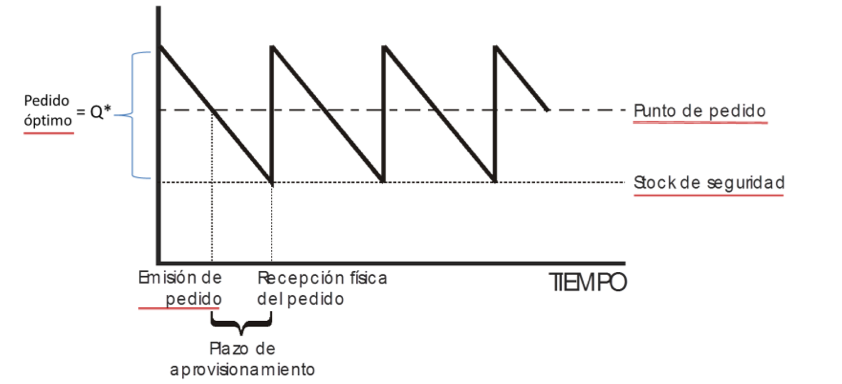
\includegraphics[width=0.8\textwidth]{img/ControlStock.png}
\caption{Ejemplo de pedidos óptimos, vía FMM.}
\label{fig:StockDeterminista}
\end{figure}

La optimización de stock tiene mucho interesante por dentro\footnote{Más que nada porque son matemáticas.}. Se trata de modelar la demanda y el comportamiento de los proveedores para encontrar el momento en el que hacer el pedido y la cantidad para minimizar costes y evitar roturas de stock. Los modelos usados pueden ser deterministas: por ejemplo, miramos las ventas por día y vemos a qué nivel de stock debemos de hacer un pedido contando con lo que tarda el proveedor, de tal forma que nos llegue el pedido justo al llegar al margen mínimo de seguridad (ver \fref{fig:StockDeterminista}).

El siguiente paso son los modelos estocásticos\footnote{Es una forma bonita de hablar de procesos aleatorios y que además parezca que sabes de qué estás hablando.}, donde tenemos en cuenta distribuciones de probabilidad para ciertas variables. Así, la demanda no es fija sino que podría venir dada por una distribución normal, y podríamos tener en cuenta la distribución del tiempo que tardan los distribuidores en traernos el pedido para así tener más claras las posibilidades de rotura de stock y poder seguir funcionando teniendo en cuenta fuentes de volatilidad.

Merece una mención el modelo \concept{Just In Time}, llevado a cabo por Toyota, por ejemplo. En lugar de mantener inventario, confían en los distribuidores para que les den los componentes en el momento en el que los necesitan, y así no tienen almacén.

\subsubsection{Valoración de stock}

La valoración del stock es otro problema, aunque menos interesante que el anterior. Cuando vendemos un plastafurbo, tenemos que ver cuánto hemos ganado con él. Y para eso necesitamos saber cuánto nos ha costado. El coste depende del coste de las materias primas y del coste de producción, costes que pueden variar a lo largo del tiempo. Así, si tenemos un almacén de \textit{stock}, cada plastafurbo tendrá un precio distinto. ¿Cuáles vendemos primero?\footnote{O, más concretamente, qué precio les ponemos. Si vendemos el plastafurbo al coste de las primeras fabricaciones, puede ser perfectamente un plastafurbo que justo acabamos de fabricar. Todo esto es sólo a nivel contable } El coste que atribuyamos a esas ventas, afectará a nuestras cuentas de beneficios (y por lo tanto a los impuestos que pagamos) pero también a la valoración de la empresa y a la fiabilidad de nuestros estados financieros.


\begin{table}[hbtp]
\centering
\begin{tabular}{l|c|c|c}
 & \textbf{FIFO} & \textbf{LIFO} & \textbf{Media} \\ \toprule
Stock plastafurbos antiguos & \multicolumn{3}{|c}{10} \\ \midrule
Coste unidad (CU) plastafurbo antiguo & \multicolumn{3}{|c}{10} \\ \midrule
Stock plastafurbos nuevos & \multicolumn{3}{|c}{10} \\ \midrule
CU plastafurbo nuevo & \multicolumn{3}{|c}{20} \\ \midrule
Ingresos por venta de 15 plastafurbos & \multicolumn{3}{|c}{400} \\ \midrule \midrule
CU de los 10 primeros plastafurbos & 10 & 20 & 15 \\ \midrule
CU de los 5 últimos plastafurbos & 20 & 10 & 15 \\ \midrule
Coste total de los 15 plastafurbos & 200 & 250 & 225 \\ \midrule
\textbf{Beneficios} & \textbf{200} & \textbf{150} & \textbf{175} \\ \midrule \midrule
CU de stock restante & 20 & 10 & 15 \\ \midrule
\textbf{Valoración stock restante} (5 plastafurbos) & \textbf{100} & \textbf{50} & \textbf{75} \\ \bottomrule
\end{tabular}
\caption{Ejemplo de los tres métodos de valoración de stock}
\label{tab:ValoracionStock}
\end{table}

Hay tres métodos para valorar el stock (ver \fref{tab:ValoracionStock} para un ejemplo combinado), y en todos los casos suponemos entorno inflacionario (el precio de todo va aumentando a lo largo del tiempo).

\paragraph{FIFO} Los primeros objetos que vendemos son los primeros que fabricamos o compramos. Así, el coste de inventario se acerca más al coste de las últimas unidades que entraron.

\paragraph{LIFO} Marcamos como vendidos los productos que más tarde hemos fabricado. La cuenta de beneficios disminuye, al igual que lo hace la valoración del stock. No tiene sentido usar este método a nivel físico: si de verdad vendemos los últimos productos fabricados y nos dejamos los más viejos, acabaremos con un almacén de plastafurbos obsoletos que nadie querrá comprar. Así, este método sólo se usa a la hora de valorar el stock, y al disminuir la cuenta de beneficios permite ahorrarnos impuestos. De hecho, esta es una de las razones por las que está prohibido en muchos países.

\paragraph{Media o media ponderada} La media o media ponderada nos dará un coste a medio camino entre el de FIFO y LIFO, de tal forma que tenemos la ventaja de pagar menos impuestos que tiene LIFO pero sin falsear del todo la valoración de stock.

\subsection{Inversión y bolsa}

La inversión en bolsa parte de un hecho fundamental, que es que las empresas tienen propietarios, en plural, y cada uno de ellos tendrá un porcentaje de propiedad. Normalmente, el porcentaje de propiedad se divide en unidades llamadas \concept[Acción]{acciones} o participaciones.

Esa propiedad puede dar lugar a diversos derechos, como por ejemplo el de recibir una parte de los beneficios de la empresa (\concept{Dividendo}) o a poder participar en la toma de decisiones de la empresa a través del \concept{Consejo\IS de accionistas}.

Monetariamente, esas participaciones tienen un valor económico, un valor que será proporcional a la valoración de la empresa. Además, esas participaciones se pueden vender y comprar. La bolsa es el mercado donde las participaciones o acciones de empresas se venden y se compran.

Como en cualquier acción de compra y venta, el precio fluctúa por la ley de la oferta y la demanda, y esas fluctuaciones de precio permiten ganar dinero (y, por supuesto, perderlo) en la bolsa a través de operaciones.

Una nota: se pueden hacer \concept{Split} y \concept{Contrasplit} cuando se quieren agrupar o dividir acciones. Por ejemplo, un contrasplit sirve cuando las acciones cotizan a muy bajo valor: se agrupan varias y se convierten en una única acción con más valor, valor que probablemente bajará luego porque ahora se podrá dividir más (con las acciones antiguas, el precio mínimo estaría a 1 céntimo por acción, que igual es muy alto).

\subsubsection{Operaciones en bolsa}

La operación más sencilla que uno puede hacer en bolsa es comprar una acción, esperar a que su valor suba porque más gente quiera comprar participaciones de la empresa (por ejemplo, si esa empresa va bien y los inversores esperan que siga así) y venderla para recoger los beneficios. Ahora bien, las cosas pueden complicarse un poco más, y de hecho la terminología cambia. A partir de ahora, consideraremos una \concept{Posición} como una inversión abierta sobre las participaciones (o \textit{stock}) de una empresa.

Es obvio que tener acciones de una empresa es una posición, de hecho se llama \concept{Posición\IS larga}\footnote{Traducido, probablemente mal, del inglés \textit{long position}.}. Cuando el valor de una empresa sube en bolsa, podemos \concept{Cerrar\IS posiciones}, esto es, vender nuestras acciones para recoger el beneficio.

Ahora bien, eso sólo nos permite ganar dinero cuando la bolsa sube, y si hemos visto las noticias sabremos que los inversores también ganan dinero cuando la bolsa baja. Para eso se usa lo que se llama una \concept{Posición\IS corta}. Hay diferentes formas de mantener este tipo de posiciones, en cualquier caso basadas en prometer acciones a un tercero por un cierto valor $P$: si la valoración de la empresa baja por debajo de ese valor, podremos comprar las  acciones a $P - ε$ y sacar un beneficio de ε.

Las posiciones en corto se pueden lograr usando préstamos: pedimos un préstamo de $n$ acciones, en ese momento valoradas a $P$ cada una. Inmediatamente, vendemos a otro inversor esas $n$ acciones al mismo precio $P$. En este momento tenemos $Pn$ en nuestra cuenta, pero debemos $n$ acciones al prestamista. Cuando el valor de la empresa baje a $P-ε$, nosotros compraremos las acciones a ese valor y se las devolveremos al prestamista\footnote{El préstamo es en acciones, no en dinero, así que hemos saldado nuestra deuda.}. Así, al venderlas al principio ganamos $Pn$, y luego las compramos por $(P-ε)n$: nuestro beneficio será de $εn$.

También se pueden usar \concept{Contratos\IS de opciones}\footnote{De nuevo probablemente mal traducido del inglés \textit{options contract}.}. Estos contratos se venden por un precio determinado, y dan derecho al comprador a la venta o a la compra de un cierto \textit{stock} de una empresa por un precio fijo $P$ en un rango de fechas determinado. Así, podemos comprar a un inversor un contrato de venta que nos da derecho a venderle $n$ acciones a $P$ cada una dentro de unos cuantos días\footnote{O el período que sea.}. Si el precio de la acción baja a $P - ε$ cuando pase ese tiempo, podremos comprar las acciones por $P - ε$ y venderlas por $P$, sacando $ε$ de beneficio por acción.

Por supuesto, esto nos puede salir mal y podemos perder dinero si el \textit{stock} sube. De hecho, si no pudiese salirnos mal no podríamos hacer este negocio con nadie porque nadie querría tirar el dinero así.

Otro tipo de operaciones financieras son los llamados \concept{Contrato\IS por diferencia (CFD)}, que necesitan de un inversor (nosotros) y un proveedor con dinero que será nuestra ``marioneta'', por así decirlo, a cambio de un módico precio. Nosotros indicamos al proveedor que queremos que compre $n$ acciones de una empresa, que ahora mismo están a precio\footnote{Habitualmente, el proveedor dice el precio $P_b$ al que él compra las acciones, que suele estar cercano a $P$ pero que no tiene por qué ser igual.} $P$. Para que haga esa operación, tendremos que pagarle un porcentaje del coste $m$. Cuando el precio de la acción suba, nosotros daremos la instrucción al proveedor de que venda esas acciones a\footnote{Al igual que con el precio de compra, el precio de venta del proveedor no tiene por qué ser el mismo que el de cotización, pero para el caso nos da lo mismo.} $P + ε$. El beneficio de la operación, $nε$, va para nosotros.

La ventaja de estas operaciones es que habiendo invertido $m·nP$ con CFDs hemos conseguido un beneficios similar al que obtendríamos invirtiendo $nP$ en el mercado normal, así que nuestras ganancias se multiplican. La parte mala es que por un lado hay comisiones por todas partes: para comprar las CFDs hay una comisión, otra por mantenerlas de un día para otro, otra por retirar el dinero... Y, por supuesto, si la valoración de la empresa baja, las pérdidas también nos las comemos íntegras nosotros, así que nos podemos encontrar con que debemos al proveedor incluso más de lo que habíamos invertido.

\subsubsection{Indicadores financieros}
\label{sec:IndicadoresFinancieros}

Para evaluar la situación de una empresa y valorar si nos conviene invertir o no, se pueden definicir ciertos indicadores que nos den una imagen de cómo está funcionando en bolsa esa empresa.

\begin{itemize}
\item \concept{Price\IS to earnings}, es el cociente de la valoración de la empresa entre los beneficios obtenidos. El valor adecuado se suele considerar entre 10 y 17, por encima puede indicar sobrevaloración (muchos beneficios para lo poco que cuesta la acción) y, análogamente, por debajo indicará infravaloración.
\item \concept{Price\IS to sales}, lo de antes pero dividiendo entre las ventas de la empresa.
\item \concept{Price\IS to book}, lo de antes pero con el \textit{book value}\index{Book!value}, que es valor de los activos tangibles (esto es, los que tienen una valoración clara, nada de patentes, copyrights o similares) menos el de los pasivos.
\item \concept{Beta}, es la relación entre el movimiento del mercado y el de la empresa: si $β = 1$, entonces eso indica que la empresa crece con el mercado. Si $β=0$, las fluctuaciones del mercado no influyen en la valoración de la empresa. El ``mercado'' suele ser un índice de empresas, como el S\&P 500.
\item \concept{Alpha}, más comúnmente \textit{weighted alpha}, parece ser una media del crecimiento a lo largo de un año dando más peso a las variaciones más cercanas al momento actual. Si es positivo, indica que la acción ha crecido a lo largo del tiempo.
\item \concept{Yield}, es el cociente de dividendos anuales entre el precio de acción.
\item \concept{Return\IS on equity}, cociente de beneficios netos entre el valor líquido de la empresa\footnote{El valor líquido es los activos menos los pasivos o, en otras palabras, la valoración bursátil más lo que la empresa tenga ahorrado.}
\item \concept{Return\IS on assets}, lo mismo de antes pero dividido entre el total de activos.
\item \concept{Earnings\IS per share (EPS)}, los beneficios de la empresa dividido entre el número total de acciones.
\end{itemize}

\section{Administración}

\subsection{Nóminas, Seguridad Social e IRPF}

Las nóminas financian al Estado a través de dos ``agencias'': la Agencia Tributaria (Hacienda) y la Tesorería General de la Seguridad Social (TGSS).

Un trabajador tiene un salario bruto mensual $S_B$, del que se deduce una cantidad $I_S$ para la TGSS y otra $I_I$ para el IRPF\footnote{Impuesto sobre la Renta de las Personas Físicas, gestionado por la Agencia Tributaria.}. Además, la empresa paga a la TGSS otra cantidad $I_{SE}$ según el salario bruto del trabajador.

\subsubsection{Seguridad Social}

\begin{table}[hbtp]
\centering
\footnotesize
\begin{tabular}{l|r|r|r}
\textbf{Contingencia} & \textbf{Empresa} & \textbf{Trabajador} & \textbf{Total} \\ \toprule
Común - Tipo general & 23.60 & 4.70 & 28.30 \\
Común - Horas extra fuerza mayor & 12.00 & 2.00 & 14.00 \\
Común - Resto horas extra & 23.60 & 4.70 & 28.30 \\ \midrule
Desempleo - Tipo general & 5.50 & 1.55 & 7.05 \\
Desempleo - Contrato temporal a tiempo completo & 6.70 & 1.60 & 8.30 \\
Desempleo - Contrato temporal a tiempo parcial & 6.70 & 1.60 & 8.30 \\ \midrule
Fondo de Garantía Salarial (FOGASA) & 0.20 & 0 & 0.20 \\ \midrule
Formación Profesional & 0.60 & 0.10 & 0.70 \\ \midrule
Accidentes de trabajo y enfermedades profesionales & ($\ast$) & 0 & ($\ast$) \\ \midrule
\end{tabular}
\caption{Tipos (en porcentaje) de cotización, separando qué porcentaje recae en la empresa y qué porcentaje en el trabajador. La parte de ($\ast$) corresponde a la tarifa de primas que varía según trabajador.}
\label{tab:TiposSegSocial}
\end{table}

Las cotizaciones a la Seguridad Social vienen reguladas por la orden ministerial correspondiente de cada año. En 2015, aparecen en la \href{http://www.boe.es/diario_boe/txt.php?id=BOE-A-2015-847}{Orden ESS/86/2015}. Los tipos de cotización se pueden ver en la \fref{tab:TiposSegSocial}.

Las contingencias para accidentes de trabajo y enfermedades profesionales dependen de la empresa y el puesto del trabajador, según la \href{http://www.seg-social.es/Internet_1/Trabajadores/CotizacionRecaudaci10777/TarifadePrimasdeATy48410/index.htm}{tarifa de primas vigente}: se aplica el porcentaje de cotización correspondiente según la actividad económica de la empresa (Cuadro I que aparece en el PDF de la tarifa de primas) salvo que el trabajador entre en alguna de las ocupaciones del Cuadro II de la tarifa de primas, en cuyo caso será el tipo del Cuadro II el que se aplique.

\paragraph{Cálculo de la aportación a la SS} Para el cálculo de la aportación, lo primero que se hace es calcular la base de cotización. Esta está conformada por el salario bruto, sin contar indemnizaciones o compensaciones de gastos\footnotemark, e incluyendo las pagas extras prorrateadas (esto es, si tenemos dos pagas extras de $x$ euros cada una, al salario bruto para un mes de $d$ días tendremos que añadirle la parte proporcional de las pagas extras, $\frac{d}{365} \cdot 2x $). De este resultado, debemos contar por separado las horas extras y aplicarles el tipo correspondiente de contingencias comunes de la \fref{tab:TiposSegSocial} según sean horas de fuerza mayor (las empleadas para prevenir o reparar siniestros o daños extraordinarios, como terremotos, incendios o similares) o no. El resto de contingencias (desempleo, FOGASA, etc) se aplican al total de salario bruto.

Un detalle a la hora de calcular la base de cotización es que hay \href{http://www.seg-social.es/Internet_1/Trabajadores/CotizacionRecaudaci10777/Basesytiposdecotiza36537/index.htm}{mínimos y máximos de cotización} según puesto y contingencia: si la base no está en ese intervalo, ya sea porque estamos por debajo o por encima, usaremos el mínimo o el máximo respectivamente a la hora de calcular la cuota.

\footnotetext{Ver \href{http://www.seg-social.es/Internet_1/PortalEducativo/Profesores/Unidad6/Cotizacionregimengeneral/Basedecotizacion/Composiciondelabasedecotizacion/index.htm}{la web de la SS} para algunos ejemplos, el \href{http://www.seg-social.es/Internet_1/Normativa/095235?ssSourceNodeId=292}{artículo 23 del Reglamento general sobre cotización y liquidación de 1995 (que supongo sigue vigente)} para el reglamento concreto y \href{http://www.seg-social.es/prdi00/groups/public/documents/binario/178628.pdf}{este boletín de la SS} para una tabla con las deducciones concretas.}

\subsubsection{IRPF}

Cada año (más concretamente, cada ejercicio fiscal), las personas físicas deben hacer la declaración de la renta\footnote{Sólo es obligatorio habiendo recibido más de 22.000 euros brutos de un pagador o más de 11.200 euros de dos pagadores, con el segundo y siguientes pagando más de 1.500 euros.} y pagar un impuesto en base a los ingresos (renta) que haya tenido.

Para evitar el susto en la declaración, las actividades económicas están sujeta a retención. Así, cuando un empleador paga a un empleado, una parte se va a Hacienda retenida en concepto de IRPF\footnotemark. Es en la declaración de la renta donde se echan cuentas y se ve si hemos pagado de más o de menos a Hacienda.

\footnotetext{\href{http://www.agenciatributaria.es/static_files/AEAT/Contenidos_Comunes/La_Agencia_Tributaria/Informacion_institucional/Campanias/IRPF_permanente/Informacion_general/Cuestiones_destacadas/reten_ingresos_cuenta_IRPF.pdf}{Aquí los tipos de retención} según la actividad económica, y aquí el \href{http://www.agenciatributaria.es/AEAT.internet/Inicio/La_Agencia_Tributaria/Campanas/Retenciones/Ejercicio_2015__hasta_11_de_julio__o_en_su_caso__31_de_julio_/Informacion_tecnica/Informacion_tecnica.shtml}{algoritmo concreto} (horrible) que usan. En la \href{http://www.agenciatributaria.es/AEAT.internet/Retenciones.shtml}{Agencia Tributaria} está el resto de información necesaria, como un simulador de retenciones.}

La cantidad a pagar a Hacienda depende de un montón de cosas\footnote{Cosas que deberían aparecer todas en la \href{https://www.boe.es/buscar/act.php?id=BOE-A-2006-20764&tn=1&vd=&p=20151030}{Ley 35/2006} sobre el IRPF y sus sucesivas modificaciones (\href{http://www.boe.es/diario_boe/txt.php?id=BOE-A-2015-7765}{la última, de 2015}.}. La base imponible se calcula como la suma de nuestros ingresos declarados (sin incluir las cotizaciones a la Seguridad Social), quitando los que estén exentos (por ejemplo, ayudas, subvenciones). De esa base imponible se quita el mínimo personal y familiar, que como mínimo es de 5.550 euros y depende de los hijos que tenga uno a su cargo, discapacidades y demás\footnote{Ver artículos 56 a 60 de la \href{https://www.boe.es/buscar/act.php?id=BOE-A-2006-20764&b=29&tn=1&p=20141128}{Ley del IRPF}.}.

Además, a partir de la reforma fiscal que entra en vigor en 2015, se añade una partida más en concepto de ``gastos generales''\footnote{Ver artículo 19.2.f) de la \href{https://www.boe.es/buscar/act.php?id=BOE-A-2006-20764&b=29&tn=1&p=20141128}{Ley del IRPF}.}, de tal forma que además del mínimo, hay que restar 2.000 euros más de la base imponible (así que pagamos menos impuestos).

\begin{table}[hbtp]
\centering
\footnotesize
\begin{tabular}{r|r|r|r|r}
\textbf{Desde} & \textbf{Hasta} & \textbf{Longitud tramo} & \textbf{Cuota íntegra} & \textbf{Tipo aplicable} \\ \toprule
0 & 12,450 & 12,450 & 0.00 & 19.5 \\
12,450 & 20,200 & 7,750 & 2,427.75 & 24.5 \\
20,200 & 34,000 & 13,800 & 4,326.50 & 30.5 \\
34,000 & 60,000 & 26,000 & 8,535.50 & 38.0 \\
60,000 & $\infty$ & $\infty$ & 18,415.50 & 46.0 \\
\end{tabular}
\caption{Tramos del IRPF para el ejercicio fiscal 2015.}
\label{tab:Tramos2015IRPF}
\end{table}

Lo que nos quede es lo que se llama la base liquidable, a la que se aplica el impuesto según la escala de la \fref{tab:Tramos2015IRPF}, aplicando a cada tramo el porcentaje correspondiente. Por ejemplo, si nuestra base liquidable 30,000 euros una vez quitado el mínimo personal, los primeros 12,450 están gravados al 19.5 \%, los siguientes 7,750 (hasta 20,200) lo están al 24.5 \% y el resto están al 30.5 \%. El porcentaje de impuesto efectivo no es por lo tanto el del tramo en el que esté tu base liquidable, sino la media ponderada según los tramos.

Lo de la cuota íntegra es simplemente una ayuda para calcularlo: la cuota íntegra de un tramo es el resultado de aplicar a todos los tramos anteriores su gravamen correspodiente, de tal forma que sólo tengas que calcular el porcentaje para lo que lleves del último tramo y sumarle la cuota íntegra.

A modo de nota, los rendimientos del ahorro tienen otro gravamen pero no nos importa demasiado.

\subsection{Facturación, ventas y cobros. IVA}

Una factura es, formalmente, un documento con toda la información de una compraventa. Lo emiten los que pueden vender, esto es, autónomos o empresas. La factura siempre ha de incluir el IVA correspondiente a lo que se venda, según los \href{http://www.agenciatributaria.es/static_files/AEAT/Contenidos_Comunes/La_Agencia_Tributaria/Segmentos_Usuarios/Empresas_y_profesionales/Novedades_IVA_2014/Nuevos_tipos_IVA.pdf}{tipos que establezca la AEAT} (principalmente hay tres: general del 21 \%, reducido del 10 \% y superreducido del 4 \%).

Dado que no sé si en algún momento hemos hablado del \concept{Impuesto\IS sobre el Valor Añadido}\index{IVA} o no, pues lo vamos a hacer ahora. El IVA es un impuesto que recae sobre el consumidor, y que gestionan los autónomos y empresas para el Estado. Cuando le vendemos un producto a un consumidor, le cobramos el precio que queramos y además le pedimos un porcentaje de ese precio en concepto de IVA. Esa cantidad va directa al Estado en la declaración trimestral del IVA.

Cuando la venta se la hacemos a otra empresa o autónomo (esto es, no a un consumidor), seguiremos cobrándole el IVA igualmente y dándoselo al Estado. El otro deberá luego deducirse esa cantidad de IVA que nos ha pagado en su declaración del IVA, para que el Estado se la devuelva\footnote{En la práctica no se devuelve, simplemente miran cuánto IVA ha pagado la empresa y cuánto ha cobrado y le ingresa a Hacienda la diferencia - normalmente, las empresas cobran más IVA que el que pagan.}.

A la pregunta sobre si se ha de facturar o no, la respuesta es sencilla. Si se trata de ingresos esporádicos, no muy grandes y a particulares, teniendo en cuenta el engorro y los costes de hacerse autónomo, lo mejor es buscar formas alternativas de declarar esos impuestos. Si no, probablemente necesites hacerte autónomo. En cualquier caso, siempre hay que declarar los ingresos y pagar los impuestos correspondientes. Y, de mi parte, si en algún momento te planteas evadir impuestos y no poner tu parte en la financiación de todos, te mando un sincero \textit{que te jodan} muy fuerte.

\subsection{Certificados digitales}

Bueno, esto no merece mucha explicación. Las administraciones públicas emiten certificados digitales (hay que pedirlo y luego personarse en la administración que corresponda con documentos que acrediten tu identidad como persona física o jurídica) para operar con ellas a través de Internet. Si no sabes lo que es un certificado electrónico o una firma digital ni cómo funcionan a estas alturas de la carrera, no es mi culpa.

\subsection{Contratos}

\begin{table}[hbtp]
\centering
\begin{tabular}{l|l|l}
\textbf{Despido} & \textbf{Días por año trabajado} & \textbf{Mensualidades máximas} \\ \toprule
Procedente & 20 & 12 \\
Disciplinario & 0 & 0 \\
Improcedente & 33 & 24 \\
Fin contrato temporal & De 8 a 12 & - \\
\end{tabular}
\caption{Tabla con las indemnizaciones por despido.}
\label{tab:Despido}
\end{table}

Los contratos pueden ser de varios tipos, principalmente fijos y temporales (estos pueden ser por obra y servicio, por tiempo...). También hay contratos de formación y de prácticas.

Una vez que se contrata a un empleado, se le puede despedir con una siguientes indemnizaciones según el tiempo que se trabaje (días por año trabajado, añadiendo la parte proporcional a los períodos inferiores a un año) y el tipo de despido, según la \fref{tab:Despido}. Describimos a continuación los tipos de despido\footnote{Ver la sección cuarta del \href{https://www.boe.es/buscar/act.php?id=BOE-A-1995-7730&tn=1&p=20151024}{Estatuto de los trabajadores}}:

\begin{itemize}
\item \concept{Despido\IS procedente}. Se extingue el contrato por ineptitud del trabajador conocida o sobrevenida después de la contratación y del período de prueba, por faltas de asistencia o por faltas de adaptación a cambios razonables en el puesto de trabajo. También se podrá efectuar un despido por causas económicas de la empresa.
\item \concept{Despido\IS disciplinario}. Se extingue el contrato por incumplimiento grave y culpable del trabajador, como faltas repetidas e injustificadas, indisciplina, ofensas verbales o física, acoso y similares.
\item \concept{Despido\IS improcedente}. Cuando se modifiquen las condiciones de trabajo del empleado sustancialmente sin respetar el artículo 41 del Estatuto de los trabajadores, falta de pago o otro incumplimiento grave del empresario (el trabajador tendrá que solicitar en el juzgado de lo social la extinción). También habrá despido improcedente si un juez lo determina así.
\end{itemize}

Además, cuando se acaba un contrato temporal, e trabajador tendrá derecho a doce días de salario por cada año de servicio\footnote{Ver \href{http://www.empleo.gob.es/es/Guia/texto/guia_7/contenidos/guia_7_16_4.htm}{la web del Ministerio de Empleo} para los detalles exactos.}.

\section{Análisis de estados financieros}

El análisis de estados financieros de una empresa implica, como su nombre indica, analizar y diseccionar el estado del dinero en una empresa. Se podrían distinguir dos ámbitos de contabilidad: por un lado, la financiera, que considera la empresa como un todo y analiza su relación con el exterior. Por otro lado, podríamos tener la contabilidad de costes que analiza cómo funciona la empresa por dentro.

\subsection{Contabilidad: Balance, PyG y caja}
\label{sec:Contabilidad}

\begin{figure}[hbtp]
\centering
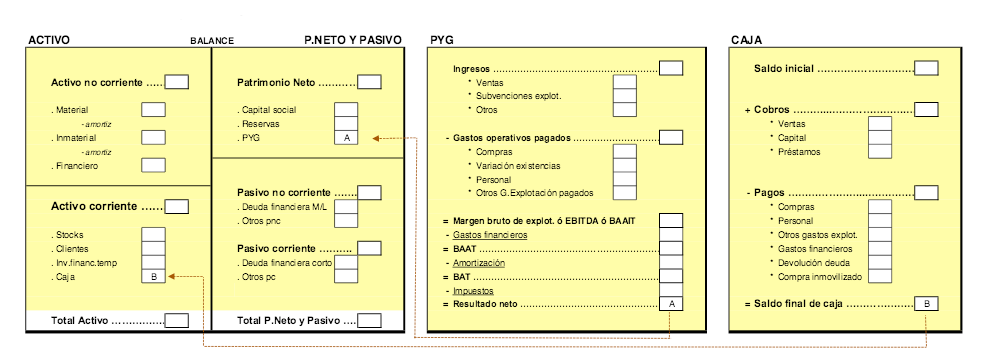
\includegraphics[width=\textwidth]{img/Balance_PyG_Caja.png}
\caption{Un ejemplo de modelo de balance, PyG y caja. Vía \href{http://maestremiranda.com/techdir/wp-content/uploads/2015/10/EF0.-Bal_PYG_Caja.pdf}{maestremiranda.com}}
\label{fig:BalancePyGCaja}
\end{figure}

Las empresas españolas están obligadas a presentar las cuentas anuales en el registro mercantil según el \href{https://www.boe.es/buscar/doc.php?id=BOE-A-2007-13023}{Plan General Contable de 2007}, corregido en la \href{https://www.boe.es/boe/dias/2009/02/10/pdfs/BOE-A-2009-2276.pdf}{Orden JUS/206/2009 del 28 de enero}.

\subsubsection{Técnica de contabilidad: Asientos}

\begin{table}[hbtp]
\centering
\begin{tabular}{r|p{5cm}||p{5cm}|l}
\textbf{Debe} & \textbf{Concepto} & \textbf{Concepto} & \textbf{Haber} \\ \toprule
1.096,25 & (640) Sueldos y salarios & (476) Organismos de la Seg. Social. acreedores & 480,81 \\
372,63 & (642) S.S. a cargo de la empresa & (4751) Hac. Pública acreedor por retenciones practicadas & 94,27 \\
 & & (465) Remuneraciones pendientes de pago & 893,8 \\ \midrule
 893,8 & (465) Remuneraciones pendientes de pago & (572) Bancos c/c & 893,8 \\ \midrule \midrule
10.000 	& (600) Compra de mercaderías & (400) Proveedores &	12.100 \\
2.100 	& (472) H.P. IVA Soportado & &  \\ \midrule
12.100 	& (400) Proveedores & (572) Bancos e instituciones bancarias &	12.100 \\ \midrule \midrule
12.100 	& (430) Clientes & 	 (700) Venta de mercaderías & 10.000 \\
 & & (477) H.P. IVA Repercutido & 2.100 \\ \midrule
12.100 & (572) Bancos c/c & (430) Clientes & 12.100 \\
 \bottomrule
\end{tabular}
\caption{Ejemplo de asientos contables. El primer asiento corresponde al pago de un salario: sale dinero de la cuenta de sueldos y salarios (lo que en el PyG aparecerá como sueldos y salarios) y de la cuenta de la seguridad social a cargo de la empresa. Ese dinero se va a la Seguridad Social (la parte de cotización de la SS de la empresa y la parte del trabajador), a la hacienda pública (el IRPF retenido) y a remuneraciones pendientes de pago. En el siguiente asiento, sacamos las remuneraciones pendientes de pago y las pagamos a través del banco. En los dos siguientes asientos, hacemos una compra de material. El tercer grupo de asientos es un ejemplo de cómo contabilizaríamos una venta pagada por entidad bancaria (si fuese al contado, en lugar de Bancos tendríamos Caja). En los dos últimos grupos de asientos, el primer asiento corresponde a cuando se hace la venta, y el segundo a cuando se hace el cobro efectivo.}
\label{tab:Asientos}
\end{table}

La técnica contable lleva la lista de asientos. Un \concept{Asiento} es simplemente el registro de una operación, porque se ve que registro no era una palabra lo suficientemente descriptiva para los economistas y contables. Cada cuenta tiene dos partes: el lado del debe (izquierdo) y el lado del haber (derecho). Esto quiere decir que una cuenta puede incrementar o aminorar su saldo según las operaciones que se realicen. Estos aumentos y disminuciones tienen un nombre: \concept{Cargo} y \concept{Abono}. \href{http://www.plangeneralcontable.com/?tit=guia-de-contabilidad-para-torpes&name=GeTia&contentId=man_ctorpes&manPage=8}{En esta página explican decentemente bien los conceptos}.

Las cuentas de donde sale y entra el dinero están definidas según el PGC\footnote{\href{https://www.boe.es/boe/dias/2007/11/20/pdfs/C00001-00152.pdf}{Plan General de Contabilidad}.}. La \fref{tab:Asientos} tiene un ejemplo con varias operaciones y su descripción.

Adicionalmente, sería relevante revisar qué pasa con las cuentas de bancos y de otros activos en general. La cuestión es que cuando una cuenta de activo aparece en el ``debe'', esta cuenta aumenta (por ejemplo, cuando ponemos la cuenta de Bancos en el debe, significa que nuestro activo por dinero en bancos aumenta), y disminuye cuando aparece en el haber. Análogamente, cuando una cuenta de pasivo aparece en el haber, su cantidad aumenta; y si aparece en el debe, su cantidad disminuye.

Al final, todos esos asientos se suman (el haber es positivo, el debe es negativo) y sale la \concept{Mayor}. El debe y el haber deberían sumar lo mismo al hacer el mayor de todas las cuentas, más que nada porque si no hemos sacado dinero de la nada.

\subsubsection{Determinación de rendimientos para el IRPF}

Cuando uno lleva a cabo una actividad económica (esto es, es autónomo), tenemos dos formas\footnotemark de estimar nuestros rendimientos netos y por lo tanto dos métodos de decirle a Hacienda cuál es nuestra base imponible sobre la que se aplican los impuestos.

\footnotetext{Esto aparece en el \href{https://www.boe.es/buscar/act.php?id=BOE-A-2006-20764}{artículo 16.2 de la ley del IRPF}, y se desarrollan los regímenes en el \href{https://www.boe.es/buscar/act.php?id=BOE-A-2007-6820}{artículo 27 del Real Decreto 439/2007}.}

Existen dos regímenes de estimación: la directa (con dos modalidades) y la objetiva.

El \concept{Régimen\IS de estimación directa simple} es el método por defecto, que sólo deja de aplicarse si renunciamos a él o si la cifra de negocio (las ventas que tenemos quitadas deducciones e IVA\footnote{Definido en el \href{http://www.boe.es/buscar/doc.php?id=BOE-A-1989-30361}{artículo 191 de un RDL derogado}, aunque parece que la cifra no ha cambiado.} supera los 600.000 euros anuales. La base imponible se calcula como los ingresos menos los gastos y deducciones, incluyendo además una deducción del 5\% del rendimiento neto del ejercicio anterior para provisiones y gastos de difícil justificación. Hay además \href{http://portal.circe.es/es-ES/emprendedor/EmpresarioIndividual/TributacionAutonomos/Paginas/AutonomoEstimacionDirectaSimplificada.aspx}{otros pequeños detalles}.

El \concept{Régimen\IS de estimación directa normal} vale cuando la cifra de negocio supera los 600.000 euros anuales de antes, y la base imponible se calcula igual pero añadiendo el autoconsumo\footnote{Ver \href{http://www.pymesyautonomos.com/fiscalidad-y-contabilidad/el-autoconsumo-de-bienes-y-servicios-tratamiento-fiscal-y-contable}{este sitio} para una explicación, básicamente es cuando el autónomo consume sus propios servicios.} a los ingresos. \href{http://portal.circe.es/es-ES/emprendedor/EmpresarioIndividual/TributacionAutonomos/Paginas/autonomoestimacionDirectaNormal.aspx}{Aquí hay más detalles}.

El \concept{Régimen\IS de estimación objetiva}\footnote{Regulado en el \href{https://www.boe.es/buscar/act.php?id=BOE-A-2007-6820}{artículo 32 del RDL 439/2007}.} se puede aplicar sólo cuando la cifra de negocio\footnote{Para la cifra de negocio debe incluirse la del cónyuge, descendientes y ascendientes que realicen actividades económicas similares.} no supera los 150.000 euros anuales (250.000 para actividades agrícolas, ganaderas y forestales), y siempre y cuando el importe de facturas emitidas a profesionales o empresarios (es decir, a consumidores habituales) no supere los 75.000 euros. Además, el volumen de las compras en bienes y servicios, excluidas las adquisiciones de inmovilizado, en el ejercicio anterior no puede superar la cantidad de 150.000 euros anuales. El cálculo de esto se hace en base a estimadores y diversos parámetros (número de empleados, de repartidores, superficie del local) según diga la normativa correspondientes. Lo malo es que estos coeficientes son pre-crisis y por lo tanto están algo desajustado de la realidad.% TODO.

\subsubsection{Balance}

Hay tres formas de afrontar la contabilidad de la empresa. La primera es la que surge al mirar el patrimonio de una empresa, que es donde vemos el activo $A$ y el pasivo $P$ (lo que se tiene y lo que se debe) y el patrimonio neto $N$. Este último a veces se denomina pasivo no exigible. En cualquier caso, las tres cantidades están relacionadas por la siguiente fórmula infinitamente complicada: \[ A - P = N\]

La \fref{fig:BalancePyGCaja} contiene una muestra de qué cuenta dentro de activos y qué dentro de pasivos. La diferencia entre activo o pasivo corriente y no corriente es sencilla: lo corriente es lo volátil, lo que está a corto plazo.

La \fref{tab:Balance} tiene un modelo abreviado del balance del Plan General Contable de 2007, relleno con los datos del siguiente ejemplo:

\begin{itemize}
\item En tesorería (cuentas corrientes) dispone de 260 (\textit{Efectivo y otros activos líquidos}).
\item Durante el ejercicio ha obtenido 10 de beneficio (\textit{PyG}).
\item Se sabe que hay una póliza de préstamo bancario por 230 (\textit{Deuda M/L}).
\item La aportación inicial de los socios fue de 100 (\textit{Capital social}).
\item A los suministradores todavía les debe 10 (letra a pagar con vencimiento 30 días) (\textit{Acreedores comerciales / proveedores}).
\item Los productos en inventario se valoran en 20 (\textit{Existencias}).
\item El activo fijo (mobiliario y ordenadores) asciende a 20 (\textit{Inmovilizado material}).
\item La cifra acumulada de beneficios retenidos es de 50 (\textit{Reservas}).
\item De las ventas realizadas le faltan por cobrar 100 (un cliente debe por mercancía no pagada) (\textit{Deudores comerciales}).
\end{itemize}

\begin{table}[hbtp]
\begin{minipage}{\textwidth}
\footnotesize
\centering
\begin{tabular}{l|c|c}
\textbf{Concepto} & \textbf{Debe} & \textbf{Haber} \\ \toprule
\multicolumn{3}{c}{\textsc{Activo} - \textbf{A) Activo no corriente}} \\ \midrule
I. Inmovilizado intangible & & - \\
II. Inmovilizado material & & 20 \\
III. Inversiones inmobiliarias & & - \\
IV. Inversiones en empresas del grupo y asociadas a largo plazo & & - \\
V. Inversiones financieras a largo plazo & & - \\
VI. Activos por impuesto diferido\footnote{Lo que el Estado nos debe de impuestos.} & & - \\
\textbf{Total activo no corriente} & & \textbf{20} \\ \midrule
\multicolumn{3}{c}{\textsc{Activo} - \textbf{B) Activo corriente}} \\ \midrule
I. Activos no corrientes para la venta & & - \\
II. Existencias & & 20 \\
III. Deudores comerciales y otras cuentas a cobrar & & 100 \\
IV. Inversiones en empresas del grupo y asociadas a corto plazo & & - \\
V. Inversiones financieras a corto plazo & & - \\
VI. Periodificaciones a corto plazo\footnote{Pagos hechos pero no devengados. Por ejemplo si se paga una póliza de seguros de dos años, la parte correspondiente al año siguiente debería ir en este epígrafe para compensar.} & & - \\
VII. Efectivo y otros activos líquidos equivalentes & & 260 \\
\textbf{Total activo corriente} & & \textbf{380} \\ \midrule
\multicolumn{3}{c}{\textsc{Patrimonio neto} - \textbf{A-1) Fondos propios}} \\ \midrule
I. Capital suscrito & & 100 \\
II. Prima de emisión\footnote{La diferencia entre el valor nominal de las acciones y el que se obtiene por ellas.} & & - \\
III. Reservas\footnote{Hay una obligación legal de manterla con cargo a los beneficios (10 \% cada año) hasta que alcance el 20\% del capital social. Sólo se podrá usar para compensar pérdidas. Si se quiere, se puede dotar por encima de ese valor, pero nunca podrá bajar del 20\% del C.S.} & & - \\
IV. Acciones y participaciones en patrimonio propias & & - \\
V. Resultados de ejercicios anteriores & - & 50 \\
VI. Otras aportaciones de socios & & - \\
VII. Resultado del ejercicio (PyG) & & 10 \\
VIII. Dividendo a cuenta & - &\\
IX. Otros instrumentos de patrimonio neto & - & - \\
\textbf{Total fondos propios} & - &  \textbf{160} \\
\textbf{A-2) Ajustes por cambio de valor} & - & - \\
\textbf{A-3) Subvenciones, donaciones y legados} & & - \\ \midrule
\multicolumn{3}{c}{\textsc{Pasivo} - \textbf{B) Pasivo no corriente}} \\ \midrule
I. Provisiones a largo plazo\footnote{Las provisiones son partidas que tendremos que pagar (sueldos, impuestos) más tarde, con importe o fecha no concretos.} & - &  \\
II. Deudas a largo plazo & 230 & \\
III. Deudas con empresas del grupo y asociadas a largo plazo & - &  \\
IV. Pasivos por impuesto diferido & - &  \\
V. Periodificaciones a largo plazo &  & \\
\textbf{Total pasivo no corriente} & \textbf{230} &  \\ \midrule
\multicolumn{3}{c}{\textsc{Pasivo} - \textbf{B) Pasivo corriente}} \\ \midrule
I. Pasivos vinculados con activos no corrientes mantenidos para la venta & - & \\
II. Provisiones a corto plazo & - & \\
III. Deudas a corto plazo  & - & \\
IV. Dedudas con empresas del grupo y asociadas a corto plazo & - & \\
V. Acreedores comerciales y otras cuentas a pagar & 10 & \\
VI. Periodificaciones a corto plazo & - & \\
\textbf{Total pasivo corriente} & \textbf{10} &  \\ \midrule
\end{tabular}
\caption{Modelo abreviado de balance relleno con el ejemplo anterior, según el Plan General Contable 2007. Se puede ver que $P = 240$, $A = 400$, $N = 160$ así que todo cuadra.}
\label{tab:Balance}
\end{minipage}
\end{table}

\paragraph{\concept{Gastos\IS Activados}} Una cosa que quizás merece la pena mencionar porque aparece en el ejemplo de balance de Terra y Jazztel de FMM. Cuando se gasta dinero en I+D, existe la posibilidad de ``activar'' esos gastos, esto es, pasarlos en el balance como activo, más concretamente inmovilizado intangible si se cumplen unas ciertas condiciones\footnote{Rentabilidad asegurada en cinco años o menos. Si son gastos de desarrollo, se puede demostrar que se van a amortizar a lo largo de más años.}. Si no se activasen, los gastos de desarrollo irían como pérdidas directamente.

¿En qué consiste exactamente esto? La idea es que se puedan distribuir los gastos de un proyecto a lo largo del tiempo. En lugar de dejar que los gastos se vayan directamente a la cuenta de beneficios y nos provoquen pérdidas, añadimos una ganancia en la cuenta 3 (Trabajos realizados por la empresa para su activo, ver la \fref{tab:PyG}) que cancele esos gastos y que aumente la partida de inmovilizado intangible en nuestro balance.

Según el PGC, los gastos de I+D deben amortizarse en un plazo de cinco años. Es decir, que podemos retrasar el momento de imputar los gastos hasta cinco años: más tarde tendrán que ir obligatoriamente como pérdidas. La cuestión es cuándo empieza ese plazo. Los gastos de investigación deben amortizarse ya desde el primer momento en el que se activan, pero los de desarrollo\footnote{La diferencia entre desarrollo o investigación es, a grandes rasgos, que el desarrollo va dirigido a una aplicación concreta y no sólo a indagar y ampliar conocimiento.} sólo se deben empezar a amortizar cuando el proyecto acaba.

Esto permite crear proyectos de desarrollo y no contar sus gastos hasta que el proyecto acaba y se puede empezar a vender. En ese caso podremos amortizar los gastos y evitar que aparezcan pérdidas cuando no deben. Por supuesto, esto admite trampas: si nunca terminamos un proyecto de desarrollo y seguimos imputando sus gastos al inmovilizado intangible, estamos enmascarando pérdidas y podemos acabar con un agujero patrimonial curioso.

\subsubsection{Pérdidas y ganancias (PyG)}

Mientras que el balance da una foto instantánea el destado de una empresa, la cuenta de pérdidas y ganancias (PyG) indica cómo varía ese estado a lo largo del tiempo. Es importante recalcar que aquí se usa el criterio de \concept{Devengo}, por el cual los ingresos y gastos computan cuando nos comprometemos a ellos y no cuando el dinero de verdad cambia de manos (por ejemplo, una factura emitida en noviembre va en las cuentas de noviembre aunque nos transfieran el dinero en diciembre).

De nuevo en la \fref{fig:BalancePyGCaja} se puede ver qué hay en cada cosa, aunque de nuevo vamos a hacer un ejemplo. Durante un ejercicio se producen los siguientes hechos:

\begin{itemize}
\item Los sueldos y salarios se elevan a 150.
\item Los intereses de la deuda ascienden a 210.
\item Los servicios generales suman 30.
\item El importe de la cifra de negocio es de 500.
\item Se han dotado 20 para recuperar activos fijos.
\item La tasa impositiva es de un 35\%.
\item Los aprovisionamientos se cifran en 70.
\item El valor del stock final supera el inicial en 60
\end{itemize}

Los resultados se pueden ver en la \fref{tab:PyG}.

\begin{table}[hbtp]
\centering
\begin{minipage}{\textwidth}
\footnotesize
\begin{tabular}{l|c|c}
\textbf{Concepto} & \textbf{Debe} & \textbf{Haber} \\ \toprule
1. Importe neto de la cifra de negocios & & 500 \\
2. Variación de existencias de productos terminados y en curso de fabricación & - & 60 \\
3. Trabajos realizados por la empresa para su activo\footnote{Por ejemplo, I+D. Ver arriba la discusión de gastos activados.} & - & \\
4. Aprovisionamientos & 70 &  \\
5. Otros ingresos de explotación\footnote{Subvenciones, donaciones y legados que financien activos o gastos de la explotación.} & & - \\
6. Gastos de personal & 150 & \\
7. Otros gastos de explotación & 30 & \\
8. Amortización del inmovilizado & - & \\
9. Imputación de subvenciones de inmovilizado no financiero\footnote{Subvenciones, legados y donaciones que financien el activo no corriente (p.e., te regalan una casa).} & - & - \\
10. Exceso de provisiones & - & \\
11. Deterioro y resultado por enajenaciones\footnote{Ventas, que los economistas hablan raro.} de inmovilizado & - & \\ \midrule
\textbf{A) Resultado de explotación} (BAAAIT) ($\sum_1^{11}$) & \textbf{250} & \textbf{560} \\ \midrule
12. Ingresos financieros & & - \\
13. Gastos financieros & 210 & \\
14. Variación de valor razonable en instrumentos financieros & - & - \\
15. Diferencias de cambio\footnote{De divisas, supongo.} & - & - \\
16. Deterioro y resultados por enajenaciones de instrumentos financieros & - & - \\ \midrule
\textbf{B) Resultado financiero} (BAAT) ($\sum_{12}^{16}$) & \textbf{210} & \textbf{0} \\ \midrule
\textbf{C) Resultado antes de impuestos} (BAT) ($A + B$) & \textbf{460} & \textbf{560} \\ \midrule
17. Impuestos sobre beneficios & 35 & \\ \midrule
\textbf{D) Resultado del ejercicio} ($C + 17$) & \textbf{495} & \textbf{560} \\ \bottomrule
\end{tabular}
\caption{Tabla de pérdidas y ganancias: el resultado final es de ganancias de 65. \href{http://www.plangeneralcontable.com/?tit=guia-del-pgc-de-pymes&name=GeTia&contentId=man_pgcpym&manPage=26}{Aquí hay} una explicación algo más detallada de los conceptos. Los \texttt{/BA+I?T/} son abreviaciones que corresponden a beneficios antes de impuestos e intereses. Hay otro \texttt{/BA+I?T/} que corresponde a los beneficios antes de amortizaciones.}
\label{tab:PyG}
\end{minipage}
\end{table}

Un concepto relevante en el PyG es la \concept{Amortización}, que permite ajustar las cuentas teniendo en cuenta la depreciación de los activos. Por ejemplo, si compramos un coche tenemos que tener en cuenta que su precio disminuye con el tiempo. La amortización implica restarle al valor de ese activo un cierto porcentaje cada año. La \href{http://www.boe.es/diario_boe/txt.php?id=BOE-A-2014-12328}{Ley 27/2014} en su artículo 12 (Capítulo II) muestra los porcentajes de amortización para cada tipo de elemento y el período máximo de años que se pueden amortizar.

El balance de pérdidas y ganancias es importante para Hacienda por el \concept{Impuesto\IS de sociedades}: es un impuesto sobre los beneficios de las empresas. En España está regulado por la Ley 27/2014, de 27 de noviembre, y es del 30\% para grandes empresas y 25\% para PYMEs, aunque luego en la práctica \href{http://www.agenciatributaria.es/AEAT.internet/Inicio/_Segmentos_/Empresas_y_profesionales/Empresas/Impuesto_sobre_Sociedades/Periodos_impositivos_iniciados_hasta_31_12_2014/Tipos_de_gravamen_aplicables_a_periodos_impositivos_iniciados_en_el_ano_2013_y_2014.shtml}{hay otros tipos contando con reducciones}. En País Vasco y Navarra, que cuentan con el concierto económico y por lo tanto Hacienda propia, los gobiernos autonómicos pueden cambiar los impuestos. Navarra mantiene los tipos del resto de España, mientras que el País Vasco \href{http://www.ogasun.ejgv.euskadi.eus/r51-341/es/contenidos/informacion/6901/es_2316/es_12215.html}{impone tipos reducidos} del 28 \% y 24 \% para grandes empresas y PYMEs respectivamente.

Hablando de \concept{PYMEs}, la definición de qué es una PYME varía según para qué queramos aplicarlo. En el caso que nos ocupa, la Agencia Tributaria, en la ley de antes que regula el IS, considera PYME (o \concept{Entidad\IS de reducida dimensión}) a aquellas que el importe neto de la cifra de negocios en el período inmediato anterior sea inferior a 10 millones de euros\footnote{Hay ciertas condiciones adicionales. Por ejemplo, si una empresa forma parte de un grupo de sociedades (definido en el \href{https://www.boe.es/buscar/act.php?id=BOE-A-1885-6627&tn=1&vd=&p=20150721}{Artículo 42 del Código de Comercio}, básicamente dos empresas pertenecen a un mismo grupo si una de ellas tiene poder sobre la otra en votos o de alguna otra forma) los beneficios que se tienen en cuenta son los de todo el grupo.}. El hecho de ser PYME o no también influye en el tipo de cuentas que deben de presentar. Para este caso, las condiciones están en el PGC\footnote{Ver \href{https://www.boe.es/boe/dias/2009/02/10/pdfs/BOE-A-2009-2276.pdf}{Orden JUS/206/2009 del 28 de enero}.}.



Hemos mencionado el \concept{Importe neto\IS de la cifra de negocios}. ``El importe de la cifra de negocios comprenderá los importes de la venta de los productos y de la prestación de servicios correspondientes a las actividades ordinarias de la Sociedad deducidas las bonificaciones y demás reducciones sobre las ventas, así como el Impuesto sobre el Valor Añadido y otros impuestos directamente relacionados con la mencionada cifra de negocios.  '' (Definición obtenida del \href{http://www.minhap.gob.es/Documentacion/Publico/NormativaDoctrina/Contabilidad%20y%20Auditoria%20de%20Empresas/Contabilidad/cifranegocA.pdf}{BOE 18/01/1992}
) Vamos, básicamente \textbf{los ingresos totales} que realmente se ingresan.

\subsubsection{Caja}

La caja es el estado más sencillo de los tres que hemos visto: refleja el flujo de dinero real en la empresa, pagos y cobros. No vamos a poner un ejemplo porque es trivial y ya llevo muchas tablas. Lo más sutil es que podemos dividir los flujos en operacionales (relacionados con la explotación, como ventas o compras a proveedores) y no operacionales (por ejemplo, ampliaciones de capital, operaciones financieras, ventas de activos no corrientes o dividendos). El resultado de esto es a veces lo que se llama el \concept{Cash-flow}.

\subsection{Circuito contable integrado}

Uno puede simplificar las cuentas en un circuito contable integrado, cuya única mención en Internet es \href{http://maestremiranda.com/techdir/wp-content/uploads/2015/10/CircuitoContable.pdf}{en maestremiranda.com}. Sencillo en cualquier caso.

\subsection{Análisis de ratios}

En la \fref{sec:IndicadoresFinancieros} veíamos algunos indicadores financieros. Para analizar el estado de una empresa usaremos algunos de estos, como el ROE (Return on Equity o rentabilidad financiera, beneficios entre recursos propios) o ROI (Return on investments, rentabilidad económica resultado de explotación entre los activos). La \fref{tab:Ratios} tiene un desglose y ejemplos de todos los ratios. En general, todos son fáciles de ver y no merecen una explicación extensa. Sólo algunas aclaraciones:

\begin{itemize}
\item La rentabilidad económica es igual al margen por la rotación (inmediato al ver las fórmulas).
\item La cobertura del inmovilizado, que tiene un nombre un poco malo, se refiere a qué porcentaje del patrimonio de la empresa está cubierto por el activo no corriente, esto es, activos que tenemos pero que no podemos usar directamente para pagar nuestras deudas. Por debajo de uno la empresa está en suspensión de pagos (no tenemos de dónde sacar dinero para pagar nuestras deudas).
\item El ratio de circulante también tiene un nombre cutre. A veces lo llaman ratio de liquidez general. En cualquier caso, sirve para ver qué porcentaje de la deuda a corto plazo se puede atender.
\item El test ácido, que de nuevo tiene un nombre feo (a veces se le llama ratio de liquidez inmediata), es similar al anterior pero se refiere sólo al dinero directo que tenemos y excluye el \textit{stock}, que tendríamos que vender si queremos usarlo para cubrir las deudas.
\item Por último, los ratios que tienen que ver con el pasivo, aunque en una primera pasada podamos pensar que es mejor tenerlos tan altos como sea posible (esto es, tener muy pocas deudas), en realidad no es así según la teoría económica: si tenemos muchos activos, podemos endeudarnos más a coste bajo e invertir más en nuestro negocio para sacar más beneficios y ganar más dinero (bienvenidos al capitalismo).
\end{itemize}

\begin{table}[hbtp]
\begin{minipage}{\textwidth}
\centering
\footnotesize
\begin{tabular}{p{3.5cm}|c|c}
\multicolumn{3}{c}{\textsc{Información}} \\ \toprule
\textbf{Concepto} & \textbf{Emp. A} & \textbf{Emp. B} \\ \toprule
\multicolumn{3}{l}{\textit{Balance}} \\ \midrule
Activo no corriente (inmovilizado) $A_P$ & 1000 & 1000 \\
Activo corriente $A_C$ & 2000 & 2000 \\
\hspace{5pt} - Stocks ($A_S$) & 1100 & 50 \\
\hspace{5pt} - Clientes & 850 & 50 \\
\hspace{5pt} - Tesorería & 50 & 1900 \\
\textbf{Total activo} ($A$) & \textbf{3000} & \textbf{3000} \\ \midrule
Recursos propios (patr. neto) ($N$) & 400 & 2600 \\
Recursos ajenos (pasivos) & 2600 & 400 \\
\hspace{5pt} - A medio/largo plazo ($P_L$) & 600 & 100 \\
\hspace{5pt} - A corto plazo ($P_C$) & 2000 & 300 \\
\textbf{Total pasivo} & \textbf{3000} & \textbf{3000} \\ \midrule
\multicolumn{3}{l}{\textit{PyG}} \\ \midrule
Ingresos $(I)$ & 60000 & 3750 \\
- Gastos operativos & 59250 & 3000 \\
= BAIT & 750 & 750 \\
- Intereses ($F$) & 234 & 36 \\
= BAT & 516 & 714 \\
- Impuestos 35 \% & 181 & 250 \\
= Resultado ($B$) & 335 & 464
\end{tabular}
~
\begin{tabular}{p{2.5cm}|c|c|c}
\multicolumn{4}{c}{\textsc{Ratios}} \\ \toprule
\textbf{Ratio} & \textbf{Fórmula} & \textbf{Emp. A} & \textbf{Emp. B} \\ \toprule
\multicolumn{4}{l}{\textit{Rentabilidad}} \\ \midrule
Financiera & $\frac{B}{N}$ & 83.7 \% & 17.8 \% \\
Económica & $\frac{BAIT}{A}$ & 25 \% & 25 \% \\
- Margen & $\frac{BAIT}{I}$ & 1.2 \% & 20 \% \\
- Rotación & $\frac{I}{A}$ & 20 & $1.25$ \\ \midrule
\multicolumn{4}{l}{\textit{Solvencia}} \\ \midrule
Activo comprometido & $\frac{P_L + P_C}{A}$ & 86.6 \% & 13.3\% \\
Cobertura inmovilizado & $\frac{N}{A_P}$ & 0.4 & 2.5 \\ \midrule
\multicolumn{4}{l}{\textit{Liquidez}} \\ \midrule
Ratio de circulante & $\frac{A_C}{P_C}$ & 1 & 6.6 \\
Test ácido & $\frac{A_C - A_S}{P_C}$ & 0.45 & 6.5 \\ \midrule
Coste de la deuda & $\frac{F}{P_L + P_C}$ & 9 \% & 9 \% \\
\end{tabular}
\caption{Análisis de estado financiero de dos empresas con ratios.}
\label{tab:Ratios}
\end{minipage}
\end{table}

\section{Viabilidad de negocios}
\section{Financiación}
\section{Evaluación de proyectos de inversión}
\section{Mercado y márketing}
\section{Recursos humanos}
\printindex
\end{document}
